\documentclass[letterpaper]{article}
\usepackage[submission]{aaai2027}
\usepackage[hyphens]{url}
\usepackage{graphicx}
\urlstyle{rm}
\def\UrlFont{\rm}
\usepackage{natbib}
\usepackage{caption}
\usepackage{booktabs}
\usepackage{amsmath}
\usepackage{array}
\frenchspacing

\pdfinfo{
/TemplateVersion (2027.1)
}

\setcounter{secnumdepth}{0}

\title{GAWorld-Bench: A Layered Validation Framework for LLM-Based Artificial Societies}
\author{Anonymous Submission}
\affiliations{}

\begin{document}
\maketitle

\begin{abstract}
Large language models make it easy to construct artificial societies whose agents remember, converse,
and react to interventions. It remains difficult to tell when such a system supports scientific inference
rather than plausible storytelling. We introduce GAWorld-Bench, a claim-centered validation framework
for LLM-based artificial societies. It separates four scientific claim layers---macro empirical fit,
emergent dynamics, counterfactual validity, and individual consistency---from a cross-cutting
reproducibility/cost gate, and requires every result to carry an evidence-provenance label. Coverage is
reported beside, rather than absorbed into, layer outcomes. We operationalize provenance, macro and
counterfactual checks, and a deterministic-mode gate; the remaining tests are specified but unimplemented.
We apply this audit retrospectively to GAWorld, an urban multiagent simulator. It reveals three failure
modes that conventional headline scores obscure: parameter recovery can be circular; two aggregation
windows yielded traffic contrasts differing by roughly 49-fold; and archived outputs from incompletely
recorded repository states are not comparable enough for causal inference. A repository headline
scorecard is also numerically identical to synthetic fixture output, while its lineage is not preserved.
We do not conclude that GAWorld predicts real populations. Instead, the case study shows how
provenance-aware, layered evaluation makes missing evidence visible and constrains the claims an
artificial-society experiment can support.
\end{abstract}

\section{Introduction}

Generative agents combine language models with memory, planning, and social interaction to produce
open-ended behavior \cite{park2023generative}. Recent systems extend this idea toward simulations of
individuals grounded in interviews and surveys \cite{park2024grounded}, while agent benchmarks evaluate
interactive task completion \cite{liu2024agentbench,ma2024agentboard} and social competence
\cite{zhou2024sotopia}. These advances create a tempting inference: if agents act plausibly, a society of
such agents can be used to study social mechanisms or policy counterfactuals.

That inference is not generally warranted. A coherent diary does not validate a population statistic;
matching a population statistic does not establish an emergent mechanism; and a directional response to
one intervention does not establish a stable counterfactual instrument. Moreover, a simulator can pass a
benchmark by recovering quantities encoded in its own parameters, or a benchmark implementation can
pass on synthetic fixtures even when no empirical model run passes. Work on agent-based models (ABMs)
has long distinguished verification, calibration, and validation \cite{sargent2013verification,
fagiolo2007critical}, but LLM-society reports often combine heterogeneous evidence into a realism score
or a small set of demonstrations.

We ask: \emph{when does an LLM-based artificial society qualify as a scientific instrument rather than a
system that generates plausible narratives?} Our answer is operational rather than philosophical. Every
claim must be paired with a validation layer, admissible evidence, provenance, and an explicit outcome:
pass, fail, or unassessed. Reproducibility is a gate, not another score that favorable dimensions can
offset.

This paper contributes:
\begin{itemize}
    \item a layered framework separating four scientific claim types from a reproducibility/cost gate;
    \item GAWorld-Bench, which operationalizes provenance, macro and counterfactual checks, coverage
    reporting, and a deterministic-mode gate while specifying the remaining tests; and
    \item a retrospective audit showing how window choice, non-comparable archives, missing tracks, and
    fixture-like scorecards can produce overconfident conclusions if evidence classes are collapsed.
\end{itemize}

Our contribution is not a claim that GAWorld is already a valid model of a real city. The audit is a
worked example of how an evaluation framework can reject unsupported conclusions and specify the
evidence still required.

\section{Related Work}

\paragraph{Generative societies and synthetic respondents.}
Generative Agents demonstrated memory, reflection, planning, and social diffusion in a small interactive
town \cite{park2023generative}. Later work grounded agents in self-reports from 1,052 participants and
evaluated held-out survey and behavioral outcomes \cite{park2024grounded}. Language models have also
been used to approximate survey samples \cite{argyle2023outofone}. This line of work motivates richer
artificial societies, but it also motivates careful limits: generated respondents need not reproduce the
experiences of real identity groups \cite{dillion2023replace,wang2025flatten}. GAWorld-Bench treats
external validity as an empirical question rather than a consequence of fluent behavior.

\paragraph{Evaluation of LLM agents.}
AgentBench evaluates reasoning and decision making across interactive environments
\cite{liu2024agentbench}; AgentBoard adds process-oriented progress measures
\cite{ma2024agentboard}; and SOTOPIA evaluates social goal achievement and interaction quality
\cite{zhou2024sotopia}. These benchmarks evaluate important capabilities of an agent. Our target is
different: a society makes claims at several levels---individual, aggregate, dynamical, and
counterfactual---whose evidence cannot be interchanged. GAWorld-Bench therefore evaluates the mapping
from claim to evidence, not only task performance.

\paragraph{Validation of simulation models.}
ABM research emphasizes transparent model description through protocols such as ODD
\cite{grimm2006odd}, empirical validation against multiple kinds of observations
\cite{windrum2007empirical,fagiolo2007critical}, and separation of verification from validation
\cite{sargent2013verification}. Generative social science further stresses explaining macro patterns from
micro rules \cite{epstein2006generative}. We adapt these principles to stochastic LLM agents and add two
practical safeguards: explicit evidence provenance and a trust gate. Placebo interventions follow the
logic of negative controls, which expose residual bias when an effect should be absent
\cite{lipsitch2010negative}.

\section{A Layered Validation Framework}

\begin{figure*}[t]
    \centering
    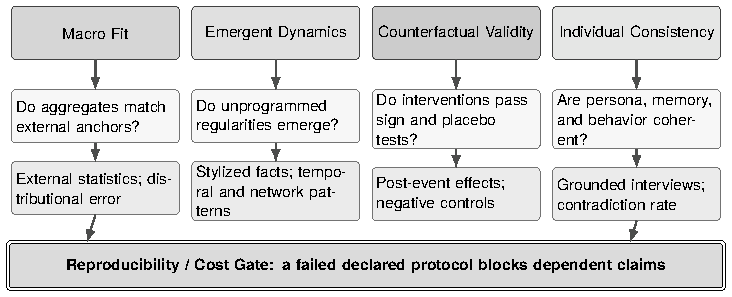
\includegraphics[width=0.88\textwidth]{figures/validation_layers.pdf}
    \caption{The framework separates four scientific claim layers and a cross-cutting engineering gate.
    Each scientific layer receives pass, fail, or unassessed status. A failed declared reproducibility
    protocol blocks dependent claims; an untested gate leaves them unverified.}
    \label{fig:layers}
\end{figure*}

Figure~\ref{fig:layers} organizes validation by the proposition being tested. The ordering is not a claim
that one layer implies another. It is a discipline for preventing evidence migration: results admissible
for one proposition cannot silently validate another.

\paragraph{L1: macro empirical fit.}
This layer asks whether simulated aggregates fall near external observations. For simulated value
$x_i$, anchor $a_i$, and relative tolerance $\tau_i$, a bounded diagnostic is
\begin{equation}
s_i=\max\left(0,1-\frac{|x_i-a_i|}{|a_i|\tau_i}\right).
\end{equation}
The vector $(s_1,\ldots,s_k)$ should remain visible even if a mean is reported. Most importantly, every
metric is tagged as \emph{input-derived} or \emph{emergent}. Recovering a tax schedule, consumption
curve, or demographic distribution directly encoded in initialization is a software or calibration check,
not independent validation.

\paragraph{L2: emergent dynamics.}
This layer asks whether unprogrammed temporal or network regularities appear: diffusion shapes,
homophily, community formation, long-tailed wealth, or other domain-specific stylized facts. A pass
requires a preregistered statistic, tolerance, time horizon, and replication rule. A qualitative anecdote
or a pattern inferred from an initialization snapshot is insufficient.

\paragraph{L3: counterfactual validity.}
For event $e$, metric $m$, matched baseline $B$, event run $E$, and endpoint $T$, define
\begin{equation}
\Delta^{\mathrm{final}}_{e,m}=y^{E}_{m,T}-y^{B}_{m,T}.
\end{equation}
A known-sign test checks whether $\operatorname{sign}(\Delta^{\mathrm{final}}_{e,m})$ matches a direction
fixed before examining output. The endpoint is a diagnostic, not a universal estimator; an event-time
average or trajectory model may be preferable when the estimand demands it. GAWorld-Bench therefore
requires the aggregation window to be declared. A placebo event additionally requires
$|\Delta_{e,m}|<\epsilon$ for unaffected metrics. Replicated runs must report uncertainty; a single seed
can provide a case, not a significance claim.

\paragraph{L4: individual consistency.}
This layer tests whether an agent's decisions remain grounded in its profile and recorded experience.
Possible probes include traceable recall, persona agreement, cross-day contradiction rate, and behavior
under memory ablations. Fluency is not a metric. LLM judges, if used, need calibration, judge-model
sensitivity checks, and access to ground-truth traces.

\paragraph{Gate: reproducibility and cost.}
The cross-cutting gate measures reproducibility under a protocol appropriate to the simulator, together
with parse or tool failure rate, tokens, and wall-clock cost. A deterministic execution mode can require
same-seed state equality; a stochastic mode instead requires replicated distributional agreement and
uncertainty estimates. Failure of the \emph{declared} protocol blocks claims that depend on paired runs,
not every possible stochastic simulation. An untested gate yields \textsc{unverified}; a failed declared
protocol yields \textsc{untrustworthy}. Neither state can be averaged away by favorable scientific layers.

\paragraph{Three-valued outcomes and coverage.}
Each configured scientific test returns pass, fail, or unassessed; the gate separately returns
\textsc{ok}, \textsc{unverified}, or \textsc{untrustworthy}. Let $n_{\mathrm{eval}}$ be evaluated tests and
$n_{\mathrm{cfg}}$ configured tests. Coverage $c=n_{\mathrm{eval}}/n_{\mathrm{cfg}}$ is reported beside any
within-layer score but is not multiplied into it: doing so would be algebraically equivalent to imputing
missing tests as zero. Missing evidence remains N/A rather than success or failure.

\section{GAWorld-Bench}

GAWorld-Bench instantiates the framework as a filesystem audit over state histories, economy ledgers,
social traces, intervention records, and matched comparison outputs. It does not require one monolithic
dataset. Instead, it assigns every artifact one of four provenance labels before scoring:
\textsc{real}, \textsc{diagnostic}, \textsc{synthetic}, or \textsc{incomplete}.

\begin{figure*}[t]
    \centering
    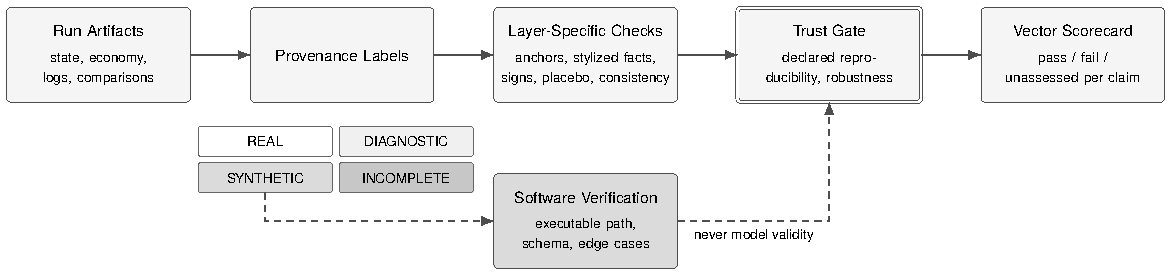
\includegraphics[width=0.96\textwidth]{figures/evidence_pipeline.pdf}
    \caption{Provenance is assigned before layer-specific checks. Synthetic fixtures are routed to
    software verification, not model validity. Incomplete artifacts remain N/A. Only admissible evidence
    reaches the trust gate and vector scorecard.}
    \label{fig:pipeline}
\end{figure*}

\begin{table}[t]
\centering
\caption{Evidence classes and permitted claims.}
\label{tab:provenance}
\footnotesize
\setlength{\tabcolsep}{3pt}
\begin{tabular}{>{\bfseries\raggedright\arraybackslash}p{0.20\columnwidth}
>{\raggedright\arraybackslash}p{0.27\columnwidth}
>{\raggedright\arraybackslash}p{0.31\columnwidth}}
\toprule
Class & Meaning & Permitted use \\
\midrule
Real & Existing simulator run & Descriptive evidence; inference only with adequate replication \\
Diagnostic & Re-analysis of real output & Measurement sensitivity and failure analysis \\
Synthetic & Fabricated structural fixture & Harness execution, schemas, and edge cases only \\
Incomplete & Missing or insufficient output & Report N/A; exclude from aggregates \\
\bottomrule
\end{tabular}
\end{table}

Figure~\ref{fig:pipeline} and Table~\ref{tab:provenance} make provenance a first-class part of the result.
This matters because synthetic data can legitimately verify a scoring path while saying nothing about
the simulator. GAWorld-Bench stores layer scores separately and reports coverage. The audited
implementation also emits a legacy coverage-discounted composite; we retain it only as a
non-decisional software output and do not interpret it because it conflates evidence quality with
missingness.

\paragraph{Counterfactual track.}
The implemented causal track combines known-sign interventions, placebo tests, and a deterministic-mode
subtest. The emitted report retains the components, gate state, and coverage; its legacy weighted scalar
is never sufficient to claim validity. In
multi-seed mode, a known-sign item counts as supported only if its confidence interval excludes zero and
has the preregistered sign.

\paragraph{Artifact auditability.}
The harness reads long-format state histories and comparison CSVs, records which directories are missing
required outputs, and archives human-readable reports. No LLM is needed to re-score completed artifacts.
This separation is important: model execution may be expensive and stochastic, while validation logic
should remain inspectable and deterministic.

\section{Auditing GAWorld}

\paragraph{Audit scope.}
We retrospectively inspected selected GAWorld artifacts and benchmark reports; we did not rerun the
simulator. The selection covers artifacts used by the benchmark's configured tracks plus known incomplete
emotion, network, and memory reports, but it is not a repository-wide exhaustive inventory. Because the
working tree and archived run metadata do not identify a common frozen release, the audit evaluates
admissible claim strength, not predictive accuracy or stochastic stability. Table~\ref{tab:audit}
separates scientific outcomes from the gate.

\begin{table}[t]
\centering
\caption{GAWorld evidence state under the layered audit.}
\label{tab:audit}
\footnotesize
\setlength{\tabcolsep}{3pt}
\begin{tabular}{>{\raggedright\arraybackslash}p{0.23\columnwidth}
>{\raggedright\arraybackslash}p{0.18\columnwidth}
>{\raggedright\arraybackslash}p{0.38\columnwidth}}
\toprule
Layer & Outcome & Reason \\
\midrule
Macro fit & Unassessed & Two one-agent snapshots do not estimate a population distribution \\
Emergent dynamics & Unassessed & Emotion state files absent; network report contains initialization only \\
Counterfactual & Unassessed & Single observations; archive comparability and uncertainty unavailable \\
Individual consistency & Unassessed & Only one memory treatment completed both phases \\
Repro. / cost & Unassessed & Cross-seed robustness, failure rate, and cost incomplete; gate \textsc{unverified} \\
\bottomrule
\end{tabular}
\end{table}

\paragraph{Macro fit is neither stable nor independent.}
The current economy snapshot contains one agent with Engel coefficient $0.48$ and savings rate $0.05$,
against benchmark-configured targets $0.288$ and $0.35$. An earlier real report contains another
one-agent snapshot with values $0.30$ and $0.25$. The urban Engel anchor is consistent with an official
Chinese statistic \cite{nbsc2025communique}; the savings target lacks a matched external definition and
is only an internal benchmark setting. Neither one-agent output estimates a population distribution.
Furthermore, the simulator directly parameterizes parts of consumption and saving. We therefore
classify these comparisons as implementation diagnostics, not external validation. A single
recorded conservation-audit row has zero monetary drift; this checks an invariant for that row only.

\paragraph{Aggregation windows change the conclusion.}
Table~\ref{tab:effects} reproduces existing audit reports. For a traffic restriction, the whole-run mean
difference in mobility intent was $+0.0068$, while the recorded endpoint difference was $+0.3368$---about
49 times larger. For a tax cut, economic security changed sign: $-0.0086$ for the whole-run mean versus
$+0.0201$ at the endpoint. These are not estimates of real policy effects. They demonstrate that an
unstated aggregation window can suppress or reverse a benchmark conclusion. An endpoint can itself be
noisy; the remedy is to declare the estimand and report trajectories or post-event windows, not to select
whichever statistic passes.

\begin{table*}[t]
\centering
\caption{Selected diagnostic values from existing real reports. Each row is unreplicated; no confidence
interval or policy-effect claim is warranted. ``Whole'' is the recorded whole-run mean difference and
``final'' is the recorded endpoint difference.}
\label{tab:effects}
\begin{tabular}{llrrrrl}
\toprule
Report & Intervention / metric & $\Delta_{\mathrm{whole}}$ & $\Delta_{\mathrm{final}}$ & $n$ & Expected & Audit reading \\
\midrule
2026-06-15 & Traffic / mobility intent & $+0.0068$ & $+0.3368$ & 1 & $+$ & 49-fold window sensitivity \\
2026-06-15 & Tax cut / economic security & $-0.0086$ & $+0.0201$ & 1 & $+$ & Sign changes by window \\
2026-06-20 & Layoff / economic security & $-0.0319$ & $-0.0498$ & 1 & $-$ & Expected sign in one run \\
2026-06-20 & Layoff / stress & $+0.1446$ & $+0.1717$ & 1 & $+$ & Expected sign in one run \\
2026-07-09 & Layoff / economic security & --- & $+0.0826$ & 1 & $-$ & Opposite sign in later batch \\
2026-07-09 & Layoff / stress & --- & $+0.0078$ & 1 & $+$ & Different magnitude; insufficient \\
\bottomrule
\end{tabular}
\end{table*}

\paragraph{Non-comparable archives block causal claims.}
A June 20 report gave layoff endpoint differences of $-0.0498$ for economic security and $+0.1717$ for
stress. A later batch contained one observation per intervention and gave $+0.0826$ and $+0.0078$,
respectively. The latter batch cannot produce a confidence interval despite being processed by the
multi-seed path. Code, prompts, population, provider, and matched-baseline metadata are not jointly
preserved across these reports. We therefore do not attribute the disagreement to stochastic instability;
we treat it as evidence that comparability, replication, version pinning, and uncertainty are required.

\paragraph{Synthetic success is not model success.}
The repository's current headline scorecard reports macro values near $0.29$ and $0.328$, four exact
known-sign effects ($+0.08$, $-0.12$, $+0.09$, $+0.06$), a perfect placebo, and perfect determinism.
Those values match the benchmark's synthetic-fixture generator exactly. This numeric fingerprint is
strong evidence of fixture-like output but, without a preserved generation command or input manifest,
does not by itself prove lineage. The scorecard is therefore admissible only as a software-path check and
is excluded from every claim about GAWorld. This illustrates why provenance must be recorded at creation.

\paragraph{What the audit establishes.}
The case study establishes that GAWorld-Bench can expose circular checks, measurement sensitivity,
non-comparable evidence, fixture-like fingerprints, and unassessed claims. It does not establish population
realism, emergent social laws, or policy-effect accuracy. This distinction is the intended output of a
validation instrument.

\section{Limitations, Ethics, and Reproducibility}

\paragraph{Limitations.}
GAWorld is one case study, and several proposed tracks are not yet implemented. The audit is
retrospective and spans changing code and configurations; this makes it useful for provenance diagnosis
but unsuitable for comparing model versions. Known-sign tests are coarse and can reward hard-coded
responses unless paired with mechanism ablations and unseen interventions. Endpoint effects can be
unstable, and placebo thresholds require domain justification. The framework still needs evaluation
across other artificial-society platforms and calibration of its decision rules.

\paragraph{Ethical statement.}
Artificial societies can help debug hypotheses before costly field work, but they can also launder model
bias into apparently quantitative policy advice. Synthetic agents do not consent, experience harm, or
represent affected communities. Their outputs should not replace empirical data or stakeholder
participation, especially for high-impact decisions. Provenance labels and unassessed states reduce, but
do not eliminate, this risk. We therefore disclose negative and missing results and avoid claims about the
modeled policies themselves.

\paragraph{Reproducibility statement.}
The audit maps each reported number to an archived CSV, JSON, or Markdown report. The package records
artifact paths and hashes, aggregation definitions, and the distinction between source artifacts and
derived diagnostics. Its offline commands verify selected extractions; they do not regenerate a complete
scorecard from a frozen run because the necessary lineage is absent. A supplement provides formulas,
the evidence ledger, and verification commands. Full reproduction of new
simulations would additionally require model/provider versions, prompts, seeds, and API behavior, which
the available artifacts do not completely preserve; the corresponding gate remains unverified.

\section{Conclusion}

LLM-based artificial societies need validation organized around claims, not plausibility. GAWorld-Bench
separates evidence layers, records coverage, preserves provenance, and gates paired scientific claims on
a declared reproducibility protocol. Its GAWorld audit shows that these safeguards change what can
responsibly be concluded: several attractive headline results are diagnostics or fixture-like, while the empirical
tracks remain incomplete or non-comparable. Making that boundary explicit is progress. Future work should
complete multi-seed, placebo, mechanism-ablation, persona-grounding, and cost evaluations across
multiple platforms.

\bibliography{references}

\end{document}
